\chapter{Fundamentação teórica}

Neste capítulo vamos apresentar os fundamentos teóricos utilizados neste trabalho acerca de proteínas e aprendizado por reforço profundo. 


\section{Proteína}
Uma proteína é uma macromolécula biológica composta por cadeias de aminoácidos. 
Constituem a maior parte da massa seca de uma célula, podendo desempenhar funções enzimáticas, estruturais,
imunológicas, de transporte, entre outras (\cite{Bio}). 

Existem milhares de proteínas diferentes em uma célula,
onde cada uma é composta por uma sequência distinta dos 20 tipos de aminoácidos encontrados na natureza,
unidos através de ligações peptídicas.
Por conta disto, as proteínas são também conhecidas como polipeptídeos (\cite{Bio}). 

A cadeia polipeptídica é composta por três componentes: a cadeia principal,
as cadeias laterais e as ligações peptídicas.
A cadeia principal é também referida como o esqueleto da proteína e
é definida como uma série repetitiva e encadeada de átomos de carbono,
nitrogénio e oxigénio. Anexadas a cadeia principal, encontram-se as cadeias laterais. 
Estas não estão envolvidas nas ligações peptídicas e são responsáveis por caracterizar as principais propriedades da proteína \cite{Bio}. 

\begin{figure}[H]
     \centering
     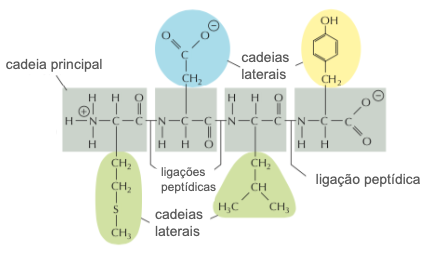
\includegraphics[width=0.6\textwidth]{figuras/ProteinBackbone.png}
     \caption{Componentes de uma proteína}
\end{figure}

\begin{figure}[H]
     \centering
     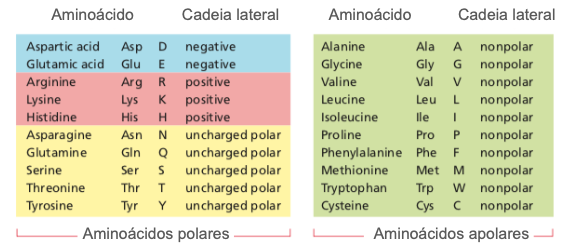
\includegraphics[width=0.7\textwidth]{figuras/20Aminoacidos.png}
     \caption[Aminiácidos]{Cada aminoácido tem uma abreviação de uma ou três letras - figura 3-2 adaptada \cite{Bio}.}
\end{figure}


\subsection{Estrutura proteíca}

A função de uma proteína está intimamente relacionada à sua estrutura tridimensional,
que é formada principalmente a partir das interações entre as cadeias laterais e móleculas encontradas no meio físico ao qual
a proteína está inserida. Devido a essas interações, a maioria das proteínas assume uma estrutura tridimensional única,
que é determinada pela ordem dos aminoácidos na sequência. 
A conformação final tende a ser aquela que possui a menor energia livre (\cite{Bio}).
Por energia livre entende-se como à energia potencial total do sistema molecular que inclui a proteína e seu meio circundante. 
Essa energia é uma medida termodinâmica que combina componentes de energia entálpica (relacionada a ligações químicas e interações eletrostáticas) 
e entropia (relacionada à desordem ou ao número de configurações possíveis das moléculas).

\cite{Bio} explica que a polaridade das cadeias laterais desempenham um papel importante na predição estrutural da proteína. 
As cadeias não polares (hidrofóbicas) tendem a se agrupar no interior da molécula, 
evitando contato com a água. 
Já as polares tendem a se dispor perto da superfície da molécula,
onde podem formar ligações de hidrogênio com a água e outras moléculas polares. 

\begin{figure}[H]
     \centering
     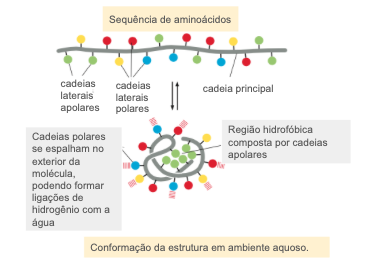
\includegraphics[width=0.6\textwidth]{figuras/ConformacaoProteica.png}
     \caption[Exemplo de conformação protéica]{Exemplo de conformação protéica \cite{Bio} - adaptado}
     %\label{Label de referência para a imagem}
\end{figure}


\subsection{O Fator IX}
O Fator IX (FIX) é uma proteína essencial para o processo de coagulação.
Quando ativado (FIXa), atua em conjunto com o Fator VIIIa (FVIIIa) para formar 
um complexo conhecido como tenase intrínseco, que é responsável por ativar o Fator X. 
Este processo é fundamental para a geração de trombina e formação de coágulos (\cite{FIX}). 
A ausência ou disfunção do FIX compromete o processo de ativação do FX,
impossibilitando uma coagulação saúdavel, o que configura a hemofilia tipo B.

\begin{figure}[H]
    \centering
    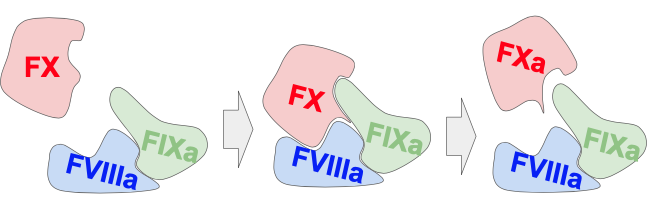
\includegraphics[width=.8\textwidth]{figuras/ativaFX.png}
    \caption{Atuação do FIXa na ativação do FX}
  \end{figure}

O FIXa é composta por diferentes domínios,
cada um desempenhando um papel essencial nas interações moleculares que permitem a formação do complexo tenase intrínseco. 
Na região N-terminal, o domínio Gla (gamma-carboxiglutâmico) é responsável por ligar o FIXa a superfícies de membranas fosfolipídicas, 
uma interação dependente de íons de cálcio, 
fundamental para posicionar o complexo de coagulação no local da lesão vascular (\cite{FIX}). 
Os domínios de fator de crescimento epidérmico (EGF1 e EGF2) desempenham funções complementares: 
o EGF1 facilita o reconhecimento de cofatores e substratos, enquanto o EGF2 interage com o domínio A3 do Fator VIIIa,
contribuindo para a montagem do complexo tenase (\cite{FIX}). 
O papel mais crítico para a estabilidade e a funcionalidade do complexo tenase reside no domínio protease,
cuja interação com o domínio A2 do FVIIIa permite a ativação conformacional necessária para uma catálise eficiente do FX.
%O domínio protease de serina contém o sítio ativo responsável pela atividade catalítica do FIXa, 
%interagindo diretamente com os domínios A2 e A3 do FVIIIa \cite{FIX}. Por conta disso,
%o domínio protease de serina é o mais relevante para a estabilidade e a eficiência catalítica do 
%complexo tenase intrínseco. 
\cite{FIX} explica que variantes do FIXa, como o FIX-Padua, que modificam o domínio protease, 
apresentam maior eficiência catalítica, destacando seu papel central no desenvolvimento de proteínas otimizadas para terapia de hemofilia.

%A formação de um complexo tenase estável depende de várias interações específicas.
%O domínio Gla do FIXa se liga ao domínio C2 do FVIIIa, promovendo a ancoragem na membrana fosfolipídica.
%Os domínios EGF1 e EGF2 interagem com os domínios A1 e A3 do FVIIIa, conferindo estabilidade adicional ao complexo.
%O papel mais crítico para a estabilidade e a funcionalidade do complexo tenase reside no domínio protease,
%cuja interação com o domínio A2 do FVIIIa permite a ativação conformacional necessária para uma catálise eficiente do FX.

\begin{figure}[H]
    \centering
    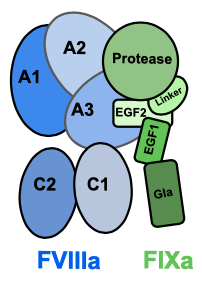
\includegraphics[width=.3\textwidth]{figuras/FIXa_FVIIIa.png}
    \caption[Interação entre FIXa e FVIIIa]{Interação entre FIXa e FVIIIa, formando o complexo tenase. Adaptação da figura 3 de \cite{FIX}}
  \end{figure}

A estrutura do domínio protease é a estrutura alvo do \textit{pipeline} de \textit{sequence design} proposto por este trabalho.  
É composta por 235 resíduos. 
Logo, o espaço de possíveis novas sequências com este tamanho, considerando 20 diferentes aminoácidos, é de $235^{20}$. 

\begin{figure}[H]
    \centering
    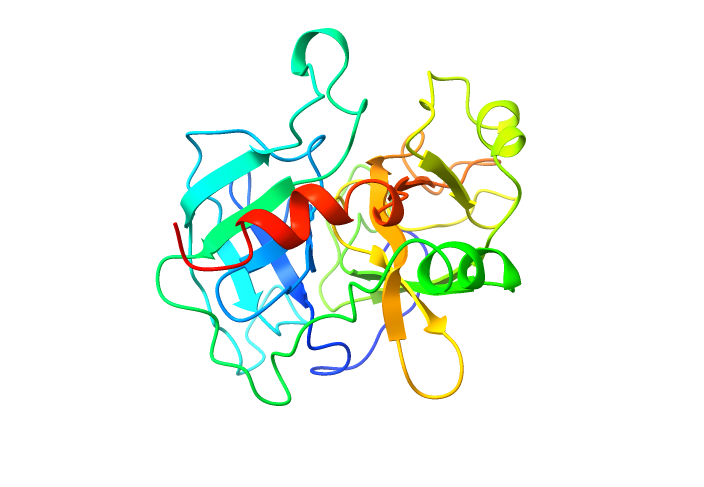
\includegraphics[width=.6\textwidth]{figuras/FIX.jpg}
    \caption{Estrutura alvo - Domínio protease do Fator IXa}
  \end{figure}

As proteínas projetadas neste estudo serão desenvolvidas para mimetizar a estrutura do domínio protease.
O objetivo é identificar, entre as variantes geradas, aquelas capazes de estabelecer interações mais estáveis com o FVIIIa,
aprimorando a estabilidade do complexo tenase intrínseco. 
Adicionalmente, espera-se que as novas estruturas apresentem um perfil imunogênico reduzido em comparação ao FIXa nativo, 
contribuindo para maior segurança e eficácia terapêutica.

\subsection{Docking}
\label{subsection:Docking} 
A análise de docking é uma técnica computacional amplamente utilizada no estudo de interações biomoleculares,
particularmente para prever a orientação e a afinidade entre duas moléculas,
como proteínas. Nesse sentido, é essencial para avaliar como uma proteína substituta do FIXa interage com o FVIIIa. 
O docking molecular simula o reconhecimento entre uma molécula receptora e outra ligante. 
No caso de interações proteína-proteína, o receptor e o ligante são ambos macromoléculas,
cujas superfícies e conformações influenciam a formação de um complexo estável.
O objetivo do docking é identificar as poses mais favoráveis termodinamicamente, ou seja, 
aquelas que minimizam a energia livre do sistema.

Durante o docking, diversas poses do ligante em relação ao receptor são geradas.
Ferramentas como RosettaDock ou AutoDock realizam essa busca, explorando translações, rotações e flexibilidade local.
Cada pose é avaliada com base em métricas energéticas, como a \textit{Contact Molecular Surface} (CMS), \textit{Interface Buried SASA} (IBSASA),
\textit{Delta Gibbs Free Energy of Binding} (DDG) e \textit{Spatial Aggregation Propensity Score} (SAP Score).

A CMS é uma medida desenvolvida para superar as limitações de métricas tradicionais, 
como Shape Complementarity (SC) e Delta Solvent Accessible Surface Area (Delta SASA) \cite{Docking}.
Enquanto SC analisa a complementaridade geométrica entre superfícies moleculares e 
Delta SASA calcula a área de superfície acessível ao solvente antes e depois da complexação,
ambas possuem limitações na identificação de interfaces bem empacotadas (\cite{Docking}).
Em contraste, o CMS combina a área de contato com um fator de penalização baseado na distância entre triângulos de superfície,
oferecendo uma representação mais precisa da qualidade do empacotamento na interface (\cite{Docking}).

A IBSASA é frequentemente usada para estimar a extensão de área de superfície enterrada durante a formação de um complexo proteico,
correlacionando-se com a estabilidade de ligação. 
No entanto, sozinha, essa métrica pode ser enganosa em interfaces mal organizadas, 
onde grandes áreas de contato podem não resultar em interações eficazes (\cite{Docking}). 

Por outro lado, a DDG fornece uma medida direta do quão favorável energéticamente é uma interação,
com valores mais negativos indicando maior estabilidade termodinâmica (\cite{Docking}). 
A DDG, calculada frequentemente com o software Rosetta, 
permite a otimização de sequências e conformações para maximizar a energia de ligação.

Por fim,o SAP Score avalia a presença de regiões hidrofóbicas expostas na superfície da proteína, 
utilizando a área de superfície acessível ao solvente (SASA) como referência. 
A partir dessa análise, estima-se a propensão da proteína ou do complexo formado à agregação indesejada.
Valores mais baixos de SAP indicam menor exposição de patches hidrofóbicos ao solvente,
sugerindo maior estabilidade estrutural e menor risco de agregação, o que é desejável na formação de complexos moleculares estáveis
(\cite{Docking}).


%O design de proteínas substitutas do FIX depende diretamente da eficácia dessas proteínas em formar complexos estáveis
%e funcionais com o FVIII. 
%A análise de docking não só ajuda a identificar mutações promissoras no FIX artificial,
%mas também fornece insights sobre como melhorar sua funcionalidade na cascata de coagulação.



\subsection{Resposta Imunológica}
\label{subsection:RespImuno} 

A resposta imune desencadeada por uma proteína terapêutica é um fator crítico 
que pode influenciar diretamente sua segurança e eficácia. 
No contexto de \textit{sequence design} de uma proteína substituta do FIXa,
a análise dessa resposta imune é especialmente relevante para evitar complicações associadas à formação de inibidores,
uma limitação comum no tratamento de hemofilia. 
Esses inibidores são anticorpos neutralizantes que se ligam à proteína administrada,
reduzindo sua eficácia e exigindo estratégias de tratamento alternativas mais caras e menos seguras.

A imunogenicidade está intrinsicamente relacionada à presença de epítopos imunogênicos na sequência da proteína. 
Esses epítopos são regiões específicas que se ligam a moléculas de MHC classe II em células 
que apresentam antígenos (APCs), 
facilitando a ativação de linfócitos T auxiliares (\cite{Imuno}). 
A afinidade de ligação é um fator determinante na indução da resposta imune. 
Altas afinidades entre peptídeos e MHC-II aumentam a probabilidade 
de reconhecimento imune e subsequente ativação de células T (\cite{Imuno}).

A predição de afinidade de ligação entre epítopos e MHC-II emprega ferramentas computacionais 
baseadas em aprendizado de máquina,
como o NetMHCIIpan, que simulam interações entre peptídeos derivados da proteína e uma variedade de alelos de MHC. 
A sequência da proteína é fragmentada em peptídeos sobrepostos com comprimentos típicos de 8 a 15 aminoácidos,
e a afinidade de cada peptídeo é quantificada por meio do valor de $IC_{50}$ (concentração inibitória de 50\%).
Peptídeos com valores de $IC_{50}$ baixos (($IC_{50}$ < 50 nM)) indicam maior afinidade de ligação e, portanto, 
são mais propensos a serem reconhecidos como epítopos imunogênicos (\cite{Imuno}).

Portanto, o objetivo ao projetar a proteína substituta do FIXa é não apenas otimizar a estabilidade de ligação ao FVIIIa, 
mas também evitar a apresentação de novos epítopos imunogênicos que poderiam levar à formação de inibidores. 
A redução da imunogenicidade melhora a adesão ao tratamento e reduz complicações, 
consolidando a importância da integração de predições imunológicas 
no \textit{pipeline} de desenvolvimento de proteínas terapêuticas.

%Apresentar equações/imagens ilustrativas das métricas

\subsection{Mutação}
Uma mutação no contexto de proteínas refere-se a uma modificação na sequência de aminoácidos. 
Por menor que seja esta modificação, a mutação pode acarretar em uma alteração na estrutura tridimensional da proteína,
uma vez que a ordem que os aminoácidos estão dispostos na sequência influencia diretamente na conformação da estrutura. 
Neste trabalho, vamos assumir que uma mutação consiste na substituição de apenas um aminoácido por outro na sequência. 

\subsection{Similariedade entre estruturas}
\label{subsection:TMScore}  
Para projetar proteínas semelhantes ao FIXa, é necessário definir uma métrica de similaridade entre estruturas.
Duas métricas amplamente utilizadas são o \textit{Root-Mean-Square Deviation} (RMSD) 
e o \textit{Template Modeling Score} (TM-score) (\cite{tmscore}),
cada uma com características próprias que influenciam sua adequação a diferentes cenários de comparação estrutural.

O \textbf{RMSD} é definido como a raiz quadrada da média dos quadrados das distâncias 
entre pares de átomos correspondentes em duas estruturas alinhadas:

\begin{equation}
    \text{RMSD} = \sqrt{\frac{1}{N} \sum_{i=1}^{N} d_i^2},
\end{equation}

onde \(N\) representa o número de pares de átomos alinhados e \(d_i\) é a distância entre os \(i\)-ésimos átomos nas estruturas comparadas. 
Embora seja uma métrica intuitiva, o RMSD é altamente sensível a desalinhamentos locais e não é normalizado pelo comprimento da proteína,
o que limita sua eficácia ao comparar proteínas de diferentes tamanhos.

O \textbf{TMScore}, por sua vez,
mede a similaridade estrutural global, superando limitações do RMSD. \cite{tmscore} a formulou da seguinte maneira:

\begin{equation}
    \text{TM-score} = \frac{1}{L_{\text{ref}}} \sum_{i=1}^{L_{\text{model}}} \frac{1}{1 + \left(\frac{d_i}{d_0(L_{\text{ref}})}\right)^2},
\end{equation}

onde \(L_{\text{ref}}\) é o número de resíduos na estrutura de referência,
 \(L_{\text{model}}\) é o número de resíduos no modelo comparado, 
 e \(d_i\) é a distância entre os átomos \(C_\alpha\) alinhados. 
 
 \cite{tmscore} define \(d_0\) em função de \(L_{\text{ref}}\) da seguinte maneira:

\begin{equation}
    d_0(L_{\text{ref}}) = 1.24 \times (L_{\text{ref}} - 15)^{1/3} - 1.8.
\end{equation}

Este parâmetro adapta a escala de distâncias consideradas significativas para o alinhamento estrutural,
ajustando-se ao comprimento da proteína de referência, \( L_{\text{ref}} \). 
O termo \( (L_{\text{ref}} - 15)^{1/3} \) 
reflete uma relação empírica entre o tamanho da proteína e as distâncias típicas entre resíduos alinhados,
modelando o crescimento da distância permissível conforme a proteína aumenta de tamanho.
A constante multiplicativa 1.24 e o deslocamento -1.8 também foram determinados empiricamente para fornecer 
um valor de \( d_0 \) que otimiza a correlação entre o TM-score e a percepção biológica de similaridade estrutural.
Essa função adapta o limiar de normalização das distâncias entre pares de resíduos alinhados,
garantindo que proteínas de diferentes comprimentos sejam comparadas de forma justa.
Proteínas maiores toleram distâncias absolutas maiores entre resíduos alinhados sem que o TM-score seja severamente penalizado (\cite{tmscore}).
 

O TMScore varia entre 0 e 1, onde valores próximos a 1 indicam alta similaridade topológica (\cite{tmscore}).
Se a distância entre cada par alinhado de átomos \(C_\alpha\) for igual a 0, então o TMScore é igual a 1, indicando sobreposição completa 
entre as macromoléculas. Em contra partida, quanto maiores são as distâncias, menor é o TMScore (mais próximo de 0).

Devido à sua robustez na avaliação da similaridade estrutural global e à sua interpretabilidade,
com valores limitados entre 0 e 1, adotaremos o TM-score como a métrica principal a ser otimizada neste projeto.
O cálculo desta medida será feito a partir da plataforma desenvolvida por (\cite{USalign}).


\subsection{Conservation Score}
\label{subsection:CS}
O \textit{Conservation Score} (CS) é uma métrica que estima a importância ou 
contribuição individual de cada resíduo da sequência na caracterização da estrutura da proteína.
Resíduos cruciais na estrutura da proteína tendem a ser conservados,
visto que alterações neles podem impactar significativamente a função proteíca (\cite{CS}). 
O score é obtido levando-se em conta a frequência com que certas combinações de aminoácidos 
ocorrem em proteínas homólogas ao longo da evolução das espécies (\cite{Eddy}). 
Para este trabalho, utilizamos o CS calculado pelo servidor ConsurfDB (\cite{ConsurfDB}),
tendo a estrutura do FIXa de coagulação como entrada. 

\begin{figure}[H]
    \centering
    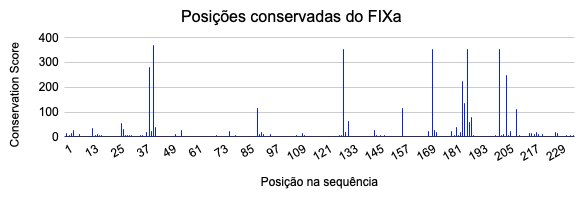
\includegraphics[width=.8\textwidth]{figuras/ConservationScore.png}
    \caption[FIXa Conservation Score]{A maior parte dos resíduos do FIXa possuem um baixo CS. Os maiores valores estão concentrados em cerca de 12 resíduos 
    espalhados ao longo da sequência.}
  \end{figure}

A identificação de posições conservadas é um aspecto fundamental ao projetar novas proteínas,
pois fornece informações essenciais para evitar mutações em regiões críticas,
preservando assim a estabilidade estrutural e a função biológica da molécula.

\subsection{Similariedade entre aminoácidos}
\label{subsection:AminoDist}
Da mesma forma que regiões com altos score de conservação devem ser evitadas, 
convém evitar mutações que substituem aminoácidos muito diferentes.
Nesse sentido, para mensurar o nível de similaridade entre os aminoácidos,
utilizamos uma métrica de distância fundamentada no trabalho de \cite{aminodist}, 
que propõe uma abordagem vetorial para representar as propriedades de cada aminoácido.
Nesse estudo, cada aminoácido foi descrito por um vetor de 544 dimensões, 
incorporando uma ampla gama de características físico-químicas e estruturais. 
A construção desses vetores foi realizada com o auxílio do pacote seqinR (\cite{seqinR}), 
uma ferramenta especializada em análise de sequências biológicas.
O pacote seqinR utiliza uma base de dados abrangente contendo propriedades como peso molecular,
hidrofobicidade, polaridade, acessibilidade à superfície, entre outras,
para derivar descritores numéricos que caracterizam as propriedades de cada aminoácido.

A partir dessa representação, \cite{aminodist} introduziu
uma matriz de distâncias, construída a partir das distâncias euclidianas de cada par 
de vetores, fornecendo uma medida quantitativa da dissimilaridade entre aminoácidos.


\begin{figure}[H]
    \centering
    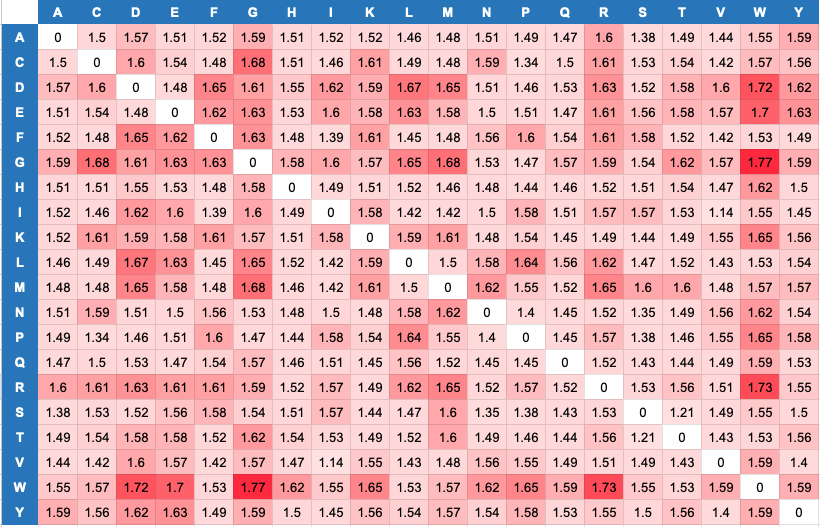
\includegraphics[width=.8\textwidth]{figuras/matrix_amino_dist.png}
    \caption[Distâncias entre aminoácidos]{Distâncias entre pares de aminoácidos \cite{aminodist}}
    \label{fig:matrixaminodist}
  \end{figure}


\section{Aprendizado por reforço profundo}
Nesta seção vamos introduzir os conceitos envolvidos no aprendizado por reforço profundo, que formam a base teórica da técnica que iremos utilizar: Proximal Policy Optimization (PPO). 
Para tal, será fornecido um contexto sobre Processo de Decisão de Markov (MDP), Redes Neurais (NN) e o método Ator-Crítico (AC). 


\subsection{Processo de Decisão de Markov}
O Processo de Decisão de Markov (MDP) é utilizado para modelar processos de forma probabilística. Ele é chamado de markoviano pois a distribuição de probabilidade de um estado depende apenas do estado anterior e da ação selecionada. Uma ação dá origem a um novo estado ao passo que promove alterações no estado atual. Um Agente seleciona cada ação com base em uma política ($\pi$) que mapeia estados a ações. Em um MDP, o processo evolui em etapas, ou \textit{steps}, à medida que o agente toma ações. A sequência de estados, desde o inicial até o final, é chamada de episódio. A qualidade de cada ação é avaliada com base no quão benéfico é o estado alcançado.
De acordo com \cite{MDP}, o MDP pode ser definido como uma tupla 
<S,A,T,R> onde:

\begin{itemize}
   \item S é o conjunto de possíveis estados;
   \item A é o conjunto de ações que interferem no processo;
   \item T :S×A×S$\rightarrow$[0,1] é uma função que quantifica a probabilidade de mudança do estado s $\in$ S para o estado $s'$ $\in$ S, dado a ação a $\in$ A selecionada. É representado por T ($s'$ |s, a);
   \item r : S × A$\rightarrow$r é uma função que mede a recompensa por selecionar a ação a $\in$ A quando o processo está no estado s $\in$ S.
 \end{itemize}

De modo a encontrar um bom $\pi$, é necessário definir uma maneira de comparar diferentes políticas. Uma técnica comum é comparar a esperança da recompensa acumulada descontada, ou Valor de Retorno (R), que cada política produziu em um mesmo episódio.

\begin{equation}
    R = E\begin{bmatrix} \sum_{k=1}^{z} \gamma ^{k-1} r_k \end{bmatrix}
\end{equation}

\noindent
Sendo z o tamanho do episódio, k o índice do \textit{step} e o $r_k$ a recompensa obtida em k. A constante $\gamma$ é um valor entre 0 e 1, chamado de fator de desconto. Ele é responsável por atribuir um peso maior a recompensas obtidas no início do episódio. 

Além disso, existem outras duas métricas importantes para se avaliar a qualidade de uma política: a Função de Valor (V) e a função de Valor da Ação (Q). A primeira estima a vantagem de estar em um estado s, calculando a esperança de R dado o estado inicial s0 = s. 

\begin{equation}
    V_\pi(s) = E[R|s_0 = s]
\end{equation}

A segunda estima a vantagem de selecionar a ação $a$ estando no estado $s$. Em outras palavras, é definida como a esperança de R dado o estado inicial e a ação inicial:

\begin{equation}
    Q_\pi(s,a) = E[R|s_0 = s, a_0 = a]
\end{equation}


Neste trabalho vamos modelar tanto a política $\pi$ quanto a Função de Valor V utilizando redes neurais profundas. 

\subsection{Redes Neurais}
Inspirado no sistema neural humano, uma rede neural artificial consiste em um conjunto de nós, chamados de neurônios, interconectados por arestas (\cite{Bishop}). 
Em geral, é organizada em camadas, que incluem três tipos: a camada de entrada, a camada oculta e a camada de saída, conforme ilustrado na figura \ref{arqNN}.

\begin{figure}[H]
     \centering
     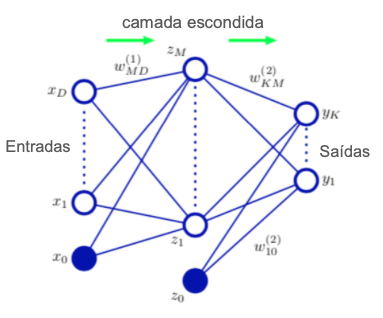
\includegraphics[width=0.6\textwidth]{figuras/RedeNeural.png}
     \caption[Arquitetura de rede neural]{Arquitetura de uma rede neural - \cite{Bishop} adaptado}
     \label{arqNN}
\end{figure}

Sinais fluem entre os neurônios através das arestas que estão associadas a um peso (w) que quantifica a sua importância. 
Nos neurônios é feito o processamento dos diversos sinais recebidos que, em seguida, aplica-se uma função, conhecida como função de ativação. 
Esta pode ser simplesmente uma combinação linear das entradas ponderadas pelos seus respectivos pesos, como pode ser função não linear como  sigmoid, 
tangente hiperbólica, entre outras (\cite{Bishop}).   

\begin{figure}[H]
     \centering
     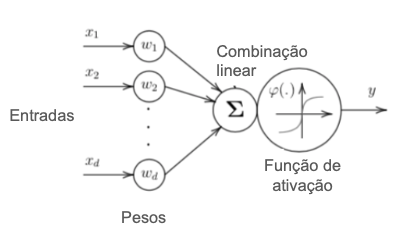
\includegraphics[width=0.6\textwidth]{figuras/ActivationFunc.png}
     \caption[Neurônio processando sinal]{Neurônio processando sinal \cite{Figueiredo}}
\end{figure}

Os pesos das arestas são ajustados durante a fase de treinamento,  de modo a orientar a rede a produzir a saída esperada para uma entrada específica. 
Nesta fase, é aplicado uma função de perda baseado na saída da rede. 
Existem diversas técnicas possíveis para minimizar a função de perda. 
Dentre elas, uma das mais tradicionais é a baseada no gradiente descendente, que atualiza os pesos conforme a equação a seguir. 

\begin{equation}
    w(t +1) = w(t) - n\nabla L(w(t)) 
\end{equation}

Onde w é o vetor de pesos, $n$ é uma constante positiva conhecida como taxa de aprendizagem, 
que quantifica o tamanho do ajuste dos parâmetros a cada iteração e $L$ é a função de perda. 
Um dos algoritmo mais utilizados para calcular o gradiente da função de perda e atualizar os parâmetros da rede é o \textit{Backpropagation} (\cite{Bishop}). 

No contexto deste trabalho, as funções de perda estarão fortemente relacionadas ao valor de Retorno R e a função de Valor V apresentadas na seção anterior. 


\subsection{Método Actor-Critic}

O método Ator-Crítico (AC) é um procedimento que tem como objetivo otimizar a política de um MDP (\cite{AC}). 
Ele é composto por dois componentes principais: o Ator e o Crítico. 
O Ator é aquele que seleciona as ações baseado nos estados, i.e, desempenha a função da política em um MDP. 
O Crítico, como o nome sugere, avalia a ação selecionada pelo Ator, estimando o vantagem de estar no estado alcançado. 
Assim, o Crítico é representado pela função de Valor do MDP. 
Tanto o Ator quanto o Crítico serão estimados por uma rede neural profunda cujos parâmetros serão ajustados utilizando a técnica \textit{Proximal Policy Optimization} (\cite{PPO}).


\subsection{PPO}

A técnica \textit{Proximal Policy Optimization} é um modelo de aprendizado por reforço profundo que define funções de perda para ajustar os pesos das redes neurais pertencentes à arquitetura do método AC (\cite{PPO}). 

Uma vez que o Crítico objetiva estimar o valor de V, o ajuste dos seus parâmetros ($W$) é feito através de um gradiente descendente a fim de minimizar o quadrado da diferença entre a saída da rede ($\hat{V}(W)$) e o V observado ($V^{obs}$) \cite{PPO}:


\begin{equation}
    L^{VF}_t(W) = (\hat{V}_t(W) - {V_t}^{obs})^2 
\end{equation}

\noindent
Uma dos principais motivações do PPO é, durante o processo de otimização do MDP, evitar atualizações de política muito grandes. 
Para isto, \cite{PPO} força com que a razão entre a política atual e a política anterior ($r_t(\Theta)$) seja limitada a um intervalo conveniente. 

\begin{equation}
    r_t(\Theta) = \frac{\pi_\Theta}{\pi_{\Theta old}}
\end{equation}

\noindent
Desta forma, para ajustar os parâmetros ($\Theta$) do Ator, \cite{PPO} define a seguinte função objetivo a ser maximizada por um gradiente ascendente:

\begin{equation}
   L^{CLIP}(\Theta) = \hat{E}_t [min(r_t (\Theta) \hat{A}_t, clip(r_t (\Theta), 1-\epsilon, 1+\epsilon) \hat{A}_t)]
\end{equation}

\noindent
Onde $\epsilon$ é uma constante que o \cite{PPO} sugere ser igual a 0.2. $\hat{A}_t$ é definido como a estimativa da função de vantagem, que corresponde ao benefício de selecionar uma ação $a$ no estado $s$, em comparação com uma seleção aleatória de uma ação no estado s. Em outras palavras, é a diferença entre Q e V:

\begin{equation}
   A = Q(s,a) - V(s)
\end{equation}

A função objetivo $L^{CLIP}(\Theta)$ é a esperança do mínimo de dois termos: $r_t(\Theta) \hat{A}_t$ e $clip(r_t (\Theta), 1-\epsilon, 1+\epsilon) \hat{A}_t$. O primeiro direciona a política a selecionar ações que maximizam a função de vantagem. O segundo é uma versão truncada do primeiro, onde é aplicado um \textit{clip} no $r_t(\Theta)$ de modo a garantir que a nova política não se distancie muito da política anterior. 

Uma vez que o aprendizado das redes do AC são dependentes entre si, \cite{PPO} sugere uma função objetivo única para treinar ambos:

\begin{equation}
   L_t ^{PPO} (\Theta) = \hat{E}_t[L_t ^{CLIP} (\Theta) - c_1 L_t ^{VF} (\Theta) + c_2 S(s_t)]
\end{equation}

Onde $c_1$ e $c_2$ são constantes e $S$ é definido por \cite{PPO} como um bônus de entropia que garante que o agente explore suficientemente o ambiente durante o treinamento.


\subsection{Escalonamento Multidimensional (MDS)}  
\label{subsection:MDS}  

O uso de técnicas de redução de dimensionalidade, como o \textit{Metric Multidimensional Scaling} (MDS),
é motivado pela necessidade de construir representações vetoriais de objetos em um espaço de menor dimensão,
preservando as distâncias definidas em uma matriz de similaridade ou dissimilaridade.
No contexto deste trabalho, utilizamos o MDS para gerar uma representação vetorial para cada aminoácido,
respeitando as distâncias previamente definidas na matriz proposta por \cite{aminodist}. 
Esta abordagem permite incorporar relações complexas de similaridade em uma forma compatível com métodos de aprendizado de máquina e
análise estrutural.  

Dado um conjunto de $n$ objetos e uma matriz de distâncias $D = (d_{ij})$,
onde cada elemento $d_{ij}$ representa a distância entre o par de objetos $i$ e $j$,
o objetivo do MDS é encontrar uma configuração vetorial $X_i = [x_{i1}, x_{i2}, ..., x_{im}]$ 
para cada objeto $i$ em um espaço de dimensão $m$,
de modo que a distância euclidiana entre $X_i$ e $X_j$ aproxime $d_{ij}$. 
O MDS busca minimizar as distâncias reais e as distâncias no espaço embutido, 
utilizando a função de perda conhecida como \textit{stress}:

\begin{equation}
    Stress(X_1, X_2, ..., X_n) = \sqrt{\sum_{i \neq j = 1}^{n} (d_{ij} - ||X_i - X_j||)^2}.
\end{equation}

A minimização desta função é geralmente realizada pelo algoritmo 
SMACOF (\textit{Scaling by MAjorizing a Complicated Function}),
que iterativamente melhora a configuração de pontos em direção a uma solução de menor \textit{stress},
garantindo uma melhor correspondência entre as distâncias calculadas e as observadas (\cite{mds}).
Embora outros métodos, como o gradiente descendente, possam ser utilizados, 
o SMACOF é amplamente preferido devido à sua eficiência e estabilidade.

Neste trabalho, 
a implementação do MDS foi realizada utilizando a biblioteca \texttt{sklearn}, 
que fornece uma solução eficiente para problemas de escala multidimensional, 
baseada nas técnicas originalmente propostas por \cite{mds}.












